\section{模型求解与结果分析}

\subsection{结果口径与评价范围}

问题一使用附件1的一天数据。其余问题均从2025年1月1日以6000 kWh初态启动，1月用于历史预测选择、残差积累和实际储能状态推进；正式填报与策略比较覆盖2月1日至12月31日，共334天、48096个10分钟时段。各策略独立推进，因此2月1日的实际初态可以不同，不能把1月运行后的库存差异隐去。

论文表格采用物理自然日时段；附件5购电页严格保留原始时间标签和列顺序，源数据与结果逐列对应，具体映射见数据处理节及附录。指定时段购电量与全天常规购电量均不含紧急购电，紧急量另列。论文中的“全天购电费”统一为全部实际支付费用。工作簿计划购电页的费用列则对应计划费用，调整购电页的费用列对应全部实际费用，避免把常规计划费用和应急费用混为一项。

四组策略的总费用、紧急需求及状态边界见表\ref{tab:annual}。其中日费用CVaR95是334个实际日费用的经验尾部均值，用于描述高费用日期，不是置信区间，也不等同于优化目标中对场景紧急费使用的CVaR90。固定电价与波动电价属于不同结算环境，不能把两者总费用之差全部归因于算法。

\begin{table}[htbp]\centering\small\caption{2025年2月1日至12月31日费用与风险结果}\label{tab:annual}
\begin{tabularx}{\linewidth}{LRRRR}\toprule
指标 & 问题2 & 问题3 & 问题4-2 & 问题4-3\\\midrule
计划费用/万元 & 1356.38 & 1373.37 & 1439.75 & 1458.54\\
调整费用/万元 & 0.00 & 23.59 & 0.00 & 22.64\\
紧急费用/万元 & 49.48 & 7.31 & 47.71 & 6.01\\
总费用/万元 & 1405.86 & 1404.27 & 1487.45 & 1487.20\\
紧急电量/万kWh & 7.99 & 1.27 & 7.51 & 0.98\\
发生紧急购电天数 & 114.00 & 86.00 & 102.00 & 82.00\\
日费用CVaR95/万元 & 7.08 & 6.64 & 8.17 & 7.76\\
最高日费用/万元 & 9.24 & 6.96 & 10.00 & 8.14\\
2月1日期初电量/kWh & 8875.19 & 8814.60 & 9251.54 & 9030.40\\
12月31日期末电量/kWh & 6164.80 & 6247.51 & 6162.13 & 6312.01\\
\bottomrule\end{tabularx}\end{table}

\subsection{问题一的确定性调度结果}

问题一的计划购电量为59482.70 kWh，购电费用为35126.95元。无储能基准在每个时段按$[L_t-R_t]_+\Delta t$购电，费用为48052.05元，因此节约12925.10元，节费率为26.90\%。全天电网侧充电量20740.67 kWh、放电量16799.94 kWh，满足$0.9\sum_tc_t=\sum_td_t/0.9$；日首和日末储电量均为6000 kWh。该结果在给定预测视为确定输入的条件下成立，不能作为未知实际出力环境的完美预测基准直接与后续方案混比。

图\ref{fig:q1}呈现两段主要储能转移：低价夜间回补电量以支持早间负荷，白天吸收光伏与低价电量以支持晚间高价负荷。早间电池没有机械地放至最低值，晚峰附近则接近物理下限，体现后续光伏补能机会与价格机会成本的共同作用。晚间结束后恢复至首态，使节费不依赖透支初始库存。10分钟尺度电价的小幅变化会导致最优充电时段出现离散跳变，题目未给出爬坡或启停约束，故不额外平滑原始最优计划。

\begin{table}[htbp]\centering\small\caption{问题1指定时段与全天购电结果（电量单位：kWh）}\label{tab:q1-purchase}
\begin{tabularx}{\linewidth}{lRlRlR}
\toprule
时间段 & 购电量 & 时间段 & 购电量 & 时间段 & 购电量\\
\midrule
10:00--10:10 & 0.00 & 12:00--12:10 & 480.41 & 14:00--14:10 & 0.00\\
16:00--16:10 & 445.43 & 18:00--18:10 & 531.89 & 20:00--20:10 & 0.00\\
\midrule
全天购电量 & 59482.70 & \multicolumn{2}{c}{全天购电费（元）} & \multicolumn{2}{r}{35126.95}\\
\bottomrule
\end{tabularx}\end{table}
\begin{table}[htbp]\centering\small\caption{问题1储能充放电及首末电量（单位：kWh）}\label{tab:q1-battery}
\begin{tabularx}{\linewidth}{lRRlRR}
\toprule
时间段 & 充电量 & 放电量 & 时间段 & 充电量 & 放电量\\
\midrule
00:00--04:00 & 4500.00 & 0.00 & 04:00--08:00 & 833.33 & 6365.84\\
08:00--12:00 & 4787.96 & 1703.00 & 12:00--16:00 & 5286.04 & 91.10\\
16:00--20:00 & 0.00 & 5780.13 & 20:00--24:00 & 5333.33 & 2859.87\\
\midrule
0:00储电量 & \multicolumn{2}{r}{6000.00} & 24:00储电量 & \multicolumn{2}{r}{6000.00}\\
\bottomrule
\end{tabularx}\end{table}
\begin{figure}[htbp]
\centering
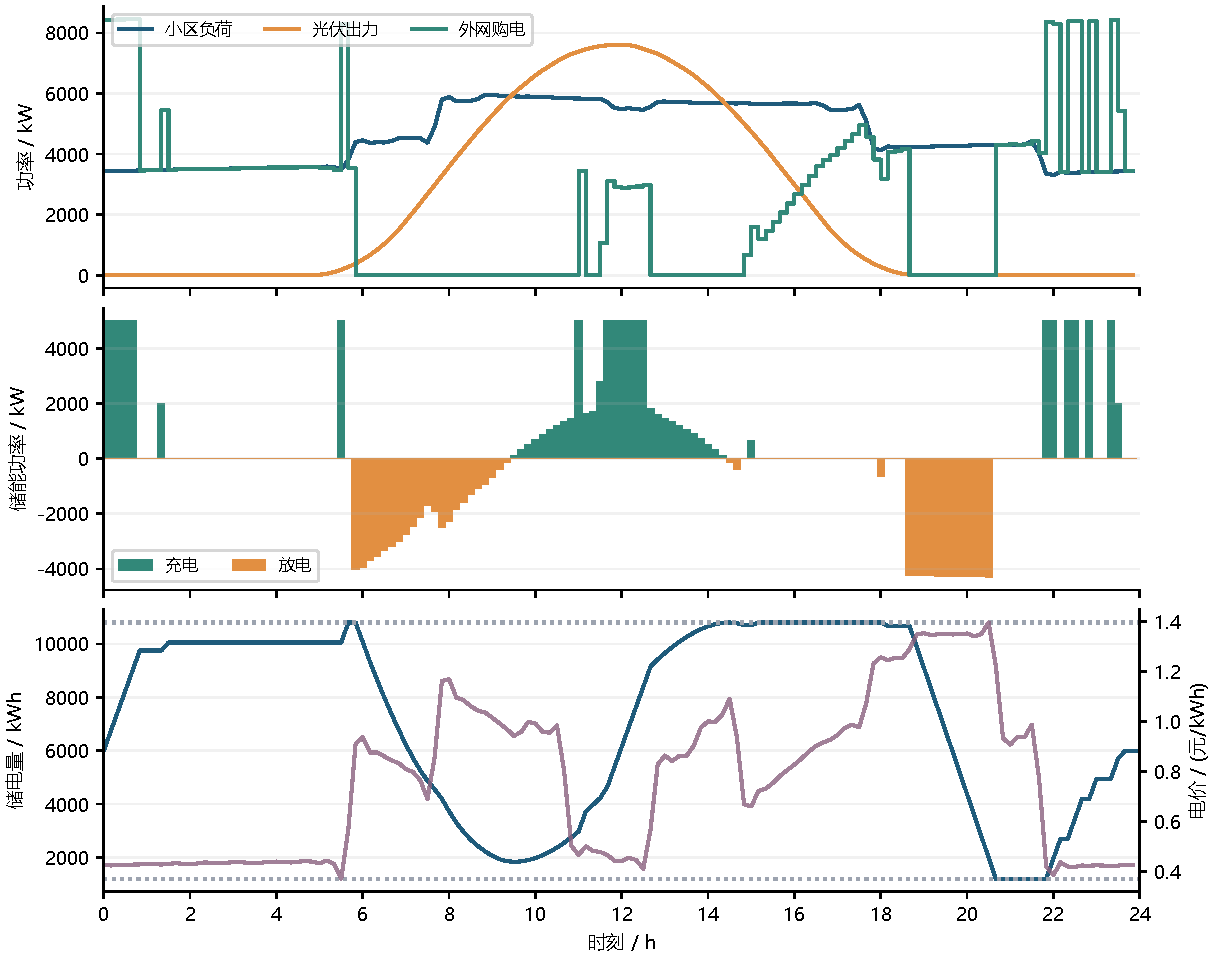
\includegraphics[width=0.94\linewidth]{figures/results/q1_dispatch.pdf}
\caption{问题一购电、充放电及储电量与电价的对应关系}
\label{fig:q1}
\end{figure}
\FloatBarrier

\subsection{问题二的风险与储能共同作用}

问题二评价期计划费用为13563772.88元，紧急费用为494809.59元，总费用14058582.47元。紧急购电量79905.90 kWh，涉及114天的550个原始10分钟时段。紧急补购后逐时满足负荷，因此这里的“紧急购电发生”表示额外昂贵补救，不能解释为失供电。

表\ref{tab:ablation}使用相同数据、评价范围与结算方式，比较无储能场景采购、点预测LP、场景期望成本、CVaR增强和参考备用增强。点预测LP费用为15918915.58元，紧急量达到614871.37 kWh，说明仅围绕均值进行精细套利，可能放大实际残差对应的五倍补购代价。主策略较该基准节省11.69\%，紧急量降低约87.00\%。无储能基准虽然采用场景采购，仍须支付18627630.00元，表明误差缓冲与电量跨时转移均具有价值。

场景期望成本模型已将费用降至14063286.32元，主策略为14058582.47元，两者总费用接近。与仅加入CVaR的14056083.78元相比，再加入参考备用多支付2498.70元，同时紧急量由90170.41降至79905.90 kWh，下降11.38\%。因此备用机制提供的是应急需求与费用之间的选择，不能把其作用夸大为无条件降低费用。

\begin{table}[htbp]\centering\small\caption{问题2的逐层对照（评价期334天）}
\label{tab:ablation}
\begin{tabularx}{\linewidth}{LRRRR}\toprule
策略 & 总费用/万元 & 紧急量/kWh & 日费CVaR95/元 & 年末电量/kWh\\\midrule
无储能+场景采购 & 1862.76 & 299833.62 & 80408.44 & 6000.00\\
点预测LP & 1591.89 & 614871.37 & 104699.88 & 5899.90\\
场景期望成本 & 1406.33 & 116065.71 & 72318.87 & 6150.47\\
场景+CVaR & 1405.61 & 90170.40 & 71037.47 & 6164.44\\
场景+CVaR+参考备用 & 1405.86 & 79905.90 & 70757.81 & 6164.80\\
\bottomrule\end{tabularx}\end{table}
\begin{table}[htbp]\centering\small
\caption{问题2指定日期购电结果（沿用题目表1布局，电量单位：kWh）}
\label{tab:q2-purchase}
\par\smallskip\textbf{2025-03-20}\par\smallskip
\begin{tabularx}{\linewidth}{lRlRlR}
\toprule
时间段 & 购电量 & 时间段 & 购电量 & 时间段 & 购电量\\
\midrule
10:00--10:10 & 0.00 & 12:00--12:10 & 634.67 & 14:00--14:10 & 0.00\\
16:00--16:10 & 485.00 & 18:00--18:10 & 692.70 & 20:00--20:10 & 0.00\\
\midrule
全天购电量 & 69564.03 & \multicolumn{2}{c}{全天购电费（元）} & \multicolumn{2}{r}{42461.59}\\
\bottomrule
\end{tabularx}
\par\smallskip\textbf{2025-06-21}\par\smallskip
\begin{tabularx}{\linewidth}{lRlRlR}
\toprule
时间段 & 购电量 & 时间段 & 购电量 & 时间段 & 购电量\\
\midrule
10:00--10:10 & 0.00 & 12:00--12:10 & 0.00 & 14:00--14:10 & 0.00\\
16:00--16:10 & 230.93 & 18:00--18:10 & 399.79 & 20:00--20:10 & 0.00\\
\midrule
全天购电量 & 40664.38 & \multicolumn{2}{c}{全天购电费（元）} & \multicolumn{2}{r}{24081.64}\\
\bottomrule
\end{tabularx}
\par\smallskip\textbf{2025-09-23}\par\smallskip
\begin{tabularx}{\linewidth}{lRlRlR}
\toprule
时间段 & 购电量 & 时间段 & 购电量 & 时间段 & 购电量\\
\midrule
10:00--10:10 & 0.00 & 12:00--12:10 & 443.93 & 14:00--14:10 & 0.00\\
16:00--16:10 & 535.12 & 18:00--18:10 & 762.12 & 20:00--20:10 & 17.80\\
\midrule
全天购电量 & 69074.66 & \multicolumn{2}{c}{全天购电费（元）} & \multicolumn{2}{r}{46508.63}\\
\bottomrule
\end{tabularx}
\par\smallskip\textbf{2025-12-21}\par\smallskip
\begin{tabularx}{\linewidth}{lRlRlR}
\toprule
时间段 & 购电量 & 时间段 & 购电量 & 时间段 & 购电量\\
\midrule
10:00--10:10 & 0.00 & 12:00--12:10 & 997.23 & 14:00--14:10 & 0.00\\
16:00--16:10 & 879.43 & 18:00--18:10 & 727.92 & 20:00--20:10 & 0.00\\
\midrule
全天购电量 & 99320.30 & \multicolumn{2}{c}{全天购电费（元）} & \multicolumn{2}{r}{64264.49}\\
\bottomrule
\end{tabularx}
\par\smallskip\parbox{\linewidth}{\footnotesize 注：问题2与4-2列示计划购电量；问题3与4-3列示最终生效的调整后常规购电量。全天购电量不含紧急购电，全天购电费含计划、调整与紧急费用。}
\end{table}

\begin{table}[htbp]\centering\small
\caption{问题2指定日期储能结果（沿用题目表2布局，单位：kWh）}
\label{tab:q2-battery}
\par\smallskip\textbf{2025-03-20}\par\smallskip
\begin{tabularx}{\linewidth}{lRRlRR}
\toprule
时间段 & 充电量 & 放电量 & 时间段 & 充电量 & 放电量\\
\midrule
00:00--04:00 & 3848.92 & 167.57 & 04:00--08:00 & 1282.09 & 4456.53\\
08:00--12:00 & 6288.36 & 2777.38 & 12:00--16:00 & 2581.36 & 417.19\\
16:00--20:00 & 260.42 & 5745.65 & 20:00--24:00 & 5531.76 & 2978.49\\
\midrule
0:00储电量 & \multicolumn{2}{r}{6707.60} & 24:00储电量 & \multicolumn{2}{r}{6140.32}\\
\bottomrule
\end{tabularx}
\par\smallskip\textbf{2025-06-21}\par\smallskip
\begin{tabularx}{\linewidth}{lRRlRR}
\toprule
时间段 & 充电量 & 放电量 & 时间段 & 充电量 & 放电量\\
\midrule
00:00--04:00 & 1059.25 & 14.93 & 04:00--08:00 & 535.52 & 2355.82\\
08:00--12:00 & 4639.89 & 0.00 & 12:00--16:00 & 0.00 & 0.00\\
16:00--20:00 & 3.17 & 4757.93 & 20:00--24:00 & 6031.16 & 2485.90\\
\midrule
0:00储电量 & \multicolumn{2}{r}{7822.98} & 24:00储电量 & \multicolumn{2}{r}{8182.20}\\
\bottomrule
\end{tabularx}
\par\smallskip\textbf{2025-09-23}\par\smallskip
\begin{tabularx}{\linewidth}{lRRlRR}
\toprule
时间段 & 充电量 & 放电量 & 时间段 & 充电量 & 放电量\\
\midrule
00:00--04:00 & 4672.35 & 162.52 & 04:00--08:00 & 798.33 & 5611.11\\
08:00--12:00 & 5607.93 & 1896.62 & 12:00--16:00 & 3859.91 & 594.11\\
16:00--20:00 & 200.18 & 5819.81 & 20:00--24:00 & 5559.88 & 2692.31\\
\midrule
0:00储电量 & \multicolumn{2}{r}{6173.75} & 24:00储电量 & \multicolumn{2}{r}{6161.95}\\
\bottomrule
\end{tabularx}
\par\smallskip\textbf{2025-12-21}\par\smallskip
\begin{tabularx}{\linewidth}{lRRlRR}
\toprule
时间段 & 充电量 & 放电量 & 时间段 & 充电量 & 放电量\\
\midrule
00:00--04:00 & 4432.44 & 92.00 & 04:00--08:00 & 1066.23 & 1424.56\\
08:00--12:00 & 6219.38 & 6304.75 & 12:00--16:00 & 5284.59 & 2220.11\\
16:00--20:00 & 7.12 & 5579.45 & 20:00--24:00 & 5642.68 & 2847.32\\
\midrule
0:00储电量 & \multicolumn{2}{r}{6654.76} & 24:00储电量 & \multicolumn{2}{r}{6521.75}\\
\bottomrule
\end{tabularx}
\end{table}

\begin{table}[htbp]\centering\small
\caption{问题2指定日期紧急购电（题目表3布局，单位：kWh）}
\label{tab:q2-emergency}
\setlength{\tabcolsep}{3pt}
\begin{tabularx}{\linewidth}{lRlRlRlR}\toprule
\multicolumn{2}{c}{2025-03-20} & \multicolumn{2}{c}{2025-06-21} & \multicolumn{2}{c}{2025-09-23} & \multicolumn{2}{c}{2025-12-21}\\
时间段 & 购电量 & 时间段 & 购电量 & 时间段 & 购电量 & 时间段 & 购电量\\\midrule
无 & 0.00 & 无 & 0.00 & 20:20--21:10 & 562.34 & 无 & 0.00\\
\midrule
合计 & 0.00 & 合计 & 0.00 & 合计 & 562.34 & 合计 & 0.00\\
\bottomrule\end{tabularx}\end{table}

四个指定日期中，9月23日20:20至21:10需紧急购电562.34 kWh，其余三个指定日期无紧急补购。这并不意味着全年其他日期没有误差风险。表\ref{tab:q2-battery}中的四小时充、放电量可以同时为正，因为它们分别累加该区间内不同10分钟时段的动作，并非同一时刻同时充放电。
\FloatBarrier

\subsection{问题三的滚动修正及预报价值}

问题三的计划费用为13733730.06元，调整费用为235908.13元，紧急费用为73088.34元，总费用14042726.52元。紧急电量下降至12685.74 kWh，涉及86天、276个10分钟时段。相对问题二，总费用仅降低0.11\%，紧急量降低84.12\%；由于两问零时光伏信息源不同，该横向差异不宜全部归为滚动优化的净贡献。

为单独考察更新机制，表\ref{tab:updates}固定问题三的零时光伏预报来源及其他参数，依次允许6时、12时和18时加入更新。相对全天不更新，四次更新策略节约168834.48元，即1.19\%，紧急电量降低83.03\%。各策略从相同1月1日初态出发，保持自身运行历史，因而这是全年可执行策略的对照，不是强制每次更新前电量相同的孤立预测实验。

6时更新首先将紧急量由74740.62 kWh降至28083.40 kWh；进一步引入12时更新，费用再降低94270.14元；加入18时更新，费用再降低52353.94元、紧急量由26491.20降至12685.74 kWh。18时以后光伏预报误差的绝对改善较小，但此时储电状态、负荷偏差与晚间高价购电机会均已发生变化，故重新优化仍有收益。这些收益不能只归因于某一份光伏预报。

\begin{table}[htbp]\centering\small\caption{问题3预报更新与反馈频率的对照}
\label{tab:updates}
\begin{tabularx}{\linewidth}{LRRRR}\toprule
策略 & 总费用/万元 & 紧急量/kWh & 日费CVaR95/元 & 年末电量/kWh\\\midrule
仅0时 & 1421.16 & 74740.62 & 70159.55 & 6247.51\\
0、6时 & 1418.94 & 28083.40 & 66393.05 & 6247.51\\
0、6、12时 & 1409.51 & 26491.20 & 66457.03 & 6247.51\\
0、6、12、18时 & 1404.27 & 12685.74 & 66381.40 & 6247.51\\
\bottomrule\end{tabularx}\end{table}
\begin{figure}[htbp]
\centering
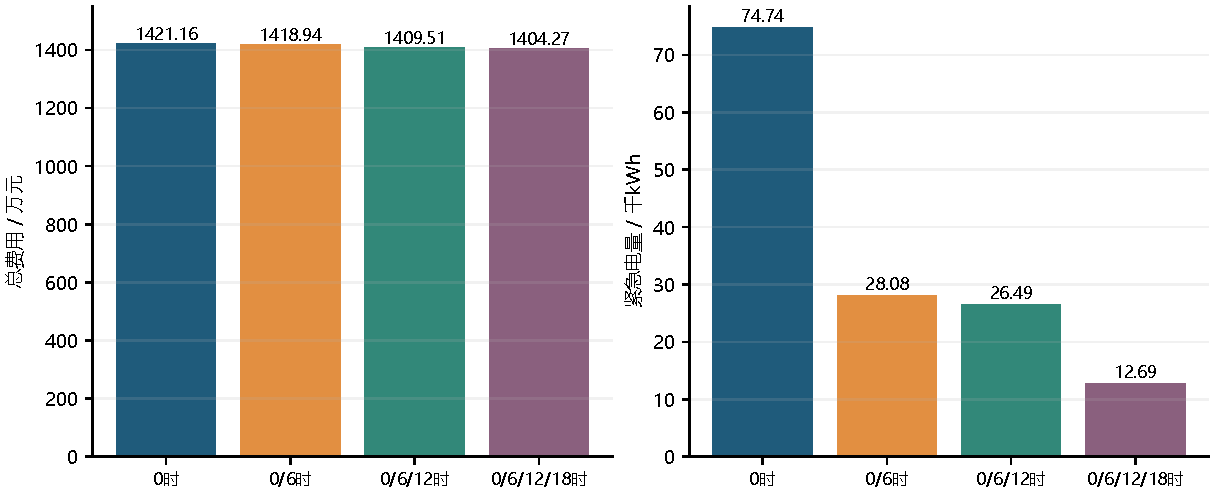
\includegraphics[width=0.98\linewidth]{figures/results/update_value.pdf}
\caption{固定零时信息源后，增加规定更新时点的费用与紧急量变化}
\label{fig:update_value}
\end{figure}

据此，在题目给定的免费预报与调度条件下，建议使用6、12、18时的更新机会。若“其他时刻”指四个规定时点之外，则附件没有提供相应预报，无法给出增加到每小时或每10分钟更新后的实测费用结论。可在新增信息可获得后，以“期望减少的紧急费用减去新增调整费”与获取预报、运行优化器的成本比较，再决定是否增设时点，不能用全天真实光伏代替不存在的高频预报。

\begin{table}[htbp]\centering\small
\caption{问题3指定日期购电结果（沿用题目表1布局，电量单位：kWh）}
\label{tab:q3-purchase}
\par\smallskip\textbf{2025-03-20}\par\smallskip
\begin{tabularx}{\linewidth}{lRlRlR}
\toprule
时间段 & 购电量 & 时间段 & 购电量 & 时间段 & 购电量\\
\midrule
10:00--10:10 & 0.00 & 12:00--12:10 & 644.57 & 14:00--14:10 & 0.00\\
16:00--16:10 & 663.46 & 18:00--18:10 & 694.45 & 20:00--20:10 & 0.00\\
\midrule
全天购电量 & 72034.34 & \multicolumn{2}{c}{全天购电费（元）} & \multicolumn{2}{r}{44213.75}\\
\bottomrule
\end{tabularx}
\par\smallskip\textbf{2025-06-21}\par\smallskip
\begin{tabularx}{\linewidth}{lRlRlR}
\toprule
时间段 & 购电量 & 时间段 & 购电量 & 时间段 & 购电量\\
\midrule
10:00--10:10 & 0.00 & 12:00--12:10 & 0.00 & 14:00--14:10 & 0.00\\
16:00--16:10 & 216.64 & 18:00--18:10 & 321.63 & 20:00--20:10 & 0.00\\
\midrule
全天购电量 & 37297.18 & \multicolumn{2}{c}{全天购电费（元）} & \multicolumn{2}{r}{22283.44}\\
\bottomrule
\end{tabularx}
\par\smallskip\textbf{2025-09-23}\par\smallskip
\begin{tabularx}{\linewidth}{lRlRlR}
\toprule
时间段 & 购电量 & 时间段 & 购电量 & 时间段 & 购电量\\
\midrule
10:00--10:10 & 0.00 & 12:00--12:10 & 467.76 & 14:00--14:10 & 0.00\\
16:00--16:10 & 590.04 & 18:00--18:10 & 786.18 & 20:00--20:10 & 5.57\\
\midrule
全天购电量 & 73151.44 & \multicolumn{2}{c}{全天购电费（元）} & \multicolumn{2}{r}{45573.45}\\
\bottomrule
\end{tabularx}
\par\smallskip\textbf{2025-12-21}\par\smallskip
\begin{tabularx}{\linewidth}{lRlRlR}
\toprule
时间段 & 购电量 & 时间段 & 购电量 & 时间段 & 购电量\\
\midrule
10:00--10:10 & 0.00 & 12:00--12:10 & 992.64 & 14:00--14:10 & 0.00\\
16:00--16:10 & 897.85 & 18:00--18:10 & 724.70 & 20:00--20:10 & 0.00\\
\midrule
全天购电量 & 99253.15 & \multicolumn{2}{c}{全天购电费（元）} & \multicolumn{2}{r}{64091.54}\\
\bottomrule
\end{tabularx}
\par\smallskip\parbox{\linewidth}{\footnotesize 注：问题2与4-2列示计划购电量；问题3与4-3列示最终生效的调整后常规购电量。全天购电量不含紧急购电，全天购电费含计划、调整与紧急费用。}
\end{table}

\begin{table}[htbp]\centering\small
\caption{问题3指定日期储能结果（沿用题目表2布局，单位：kWh）}
\label{tab:q3-battery}
\par\smallskip\textbf{2025-03-20}\par\smallskip
\begin{tabularx}{\linewidth}{lRRlRR}
\toprule
时间段 & 充电量 & 放电量 & 时间段 & 充电量 & 放电量\\
\midrule
00:00--04:00 & 3970.31 & 143.39 & 04:00--08:00 & 900.49 & 5889.37\\
08:00--12:00 & 5942.16 & 2777.38 & 12:00--16:00 & 4959.17 & 254.72\\
16:00--20:00 & 17.80 & 5636.88 & 20:00--24:00 & 5546.09 & 2972.18\\
\midrule
0:00储电量 & \multicolumn{2}{r}{6677.15} & 24:00储电量 & \multicolumn{2}{r}{6241.87}\\
\bottomrule
\end{tabularx}
\par\smallskip\textbf{2025-06-21}\par\smallskip
\begin{tabularx}{\linewidth}{lRRlRR}
\toprule
时间段 & 充电量 & 放电量 & 时间段 & 充电量 & 放电量\\
\midrule
00:00--04:00 & 852.37 & 571.84 & 04:00--08:00 & 524.05 & 4390.39\\
08:00--12:00 & 8060.49 & 0.00 & 12:00--16:00 & 0.00 & 0.00\\
16:00--20:00 & 99.66 & 4836.09 & 20:00--24:00 & 6004.38 & 2485.90\\
\midrule
0:00储电量 & \multicolumn{2}{r}{7820.38} & 24:00储电量 & \multicolumn{2}{r}{8158.10}\\
\bottomrule
\end{tabularx}
\par\smallskip\textbf{2025-09-23}\par\smallskip
\begin{tabularx}{\linewidth}{lRRlRR}
\toprule
时间段 & 充电量 & 放电量 & 时间段 & 充电量 & 放电量\\
\midrule
00:00--04:00 & 4299.55 & 80.35 & 04:00--08:00 & 823.04 & 5847.79\\
08:00--12:00 & 6293.08 & 1896.62 & 12:00--16:00 & 3657.67 & 413.77\\
16:00--20:00 & 131.83 & 5662.28 & 20:00--24:00 & 5678.17 & 3091.35\\
\midrule
0:00储电量 & \multicolumn{2}{r}{6376.64} & 24:00储电量 & \multicolumn{2}{r}{6291.47}\\
\bottomrule
\end{tabularx}
\par\smallskip\textbf{2025-12-21}\par\smallskip
\begin{tabularx}{\linewidth}{lRRlRR}
\toprule
时间段 & 充电量 & 放电量 & 时间段 & 充电量 & 放电量\\
\midrule
00:00--04:00 & 4544.08 & 36.25 & 04:00--08:00 & 961.65 & 1476.18\\
08:00--12:00 & 6423.45 & 6283.79 & 12:00--16:00 & 5219.32 & 2316.39\\
16:00--20:00 & 6.05 & 5572.83 & 20:00--24:00 & 5660.24 & 2842.53\\
\midrule
0:00储电量 & \multicolumn{2}{r}{6602.57} & 24:00储电量 & \multicolumn{2}{r}{6549.26}\\
\bottomrule
\end{tabularx}
\end{table}

\begin{table}[htbp]\centering\small
\caption{问题3指定日期紧急购电（题目表3布局，单位：kWh）}
\label{tab:q3-emergency}
\setlength{\tabcolsep}{3pt}
\begin{tabularx}{\linewidth}{lRlRlRlR}\toprule
\multicolumn{2}{c}{2025-03-20} & \multicolumn{2}{c}{2025-06-21} & \multicolumn{2}{c}{2025-09-23} & \multicolumn{2}{c}{2025-12-21}\\
时间段 & 购电量 & 时间段 & 购电量 & 时间段 & 购电量 & 时间段 & 购电量\\\midrule
无 & 0.00 & 无 & 0.00 & 20:20--20:30 & 6.38 & 无 & 0.00\\
\midrule
合计 & 0.00 & 合计 & 0.00 & 合计 & 6.38 & 合计 & 0.00\\
\bottomrule\end{tabularx}\end{table}
\begin{table}[htbp]\centering\small
\caption{问题3指定日期计划、调整与费用分解}
\begin{tabularx}{\linewidth}{lRRRRR}\toprule
日期 & 计划量/kWh & 生效量/kWh & 计划费/元 & 调整费/元 & 紧急费/元\\\midrule
2025-03-20 & 71922.07 & 72034.34 & 44073.93 & 139.82 & 0.00\\
2025-06-21 & 37292.62 & 37297.18 & 22276.77 & 6.67 & 0.00\\
2025-09-23 & 73151.44 & 73151.44 & 45530.46 & 0.00 & 43.00\\
2025-12-21 & 99253.15 & 99253.15 & 64091.54 & 0.00 & 0.00\\
\bottomrule\end{tabularx}\end{table}

图\ref{fig:seasons}显示四个指定日期的零时计划与最终常规购电；多数时段两条曲线重合，只有新增购电必要时才发生修订。9月23日仍有20:20至20:30共6.38 kWh紧急购电，相比问题二该日562.34 kWh显著减少，但不能声称完全消除了应急补救。

\begin{figure}[htbp]
\centering
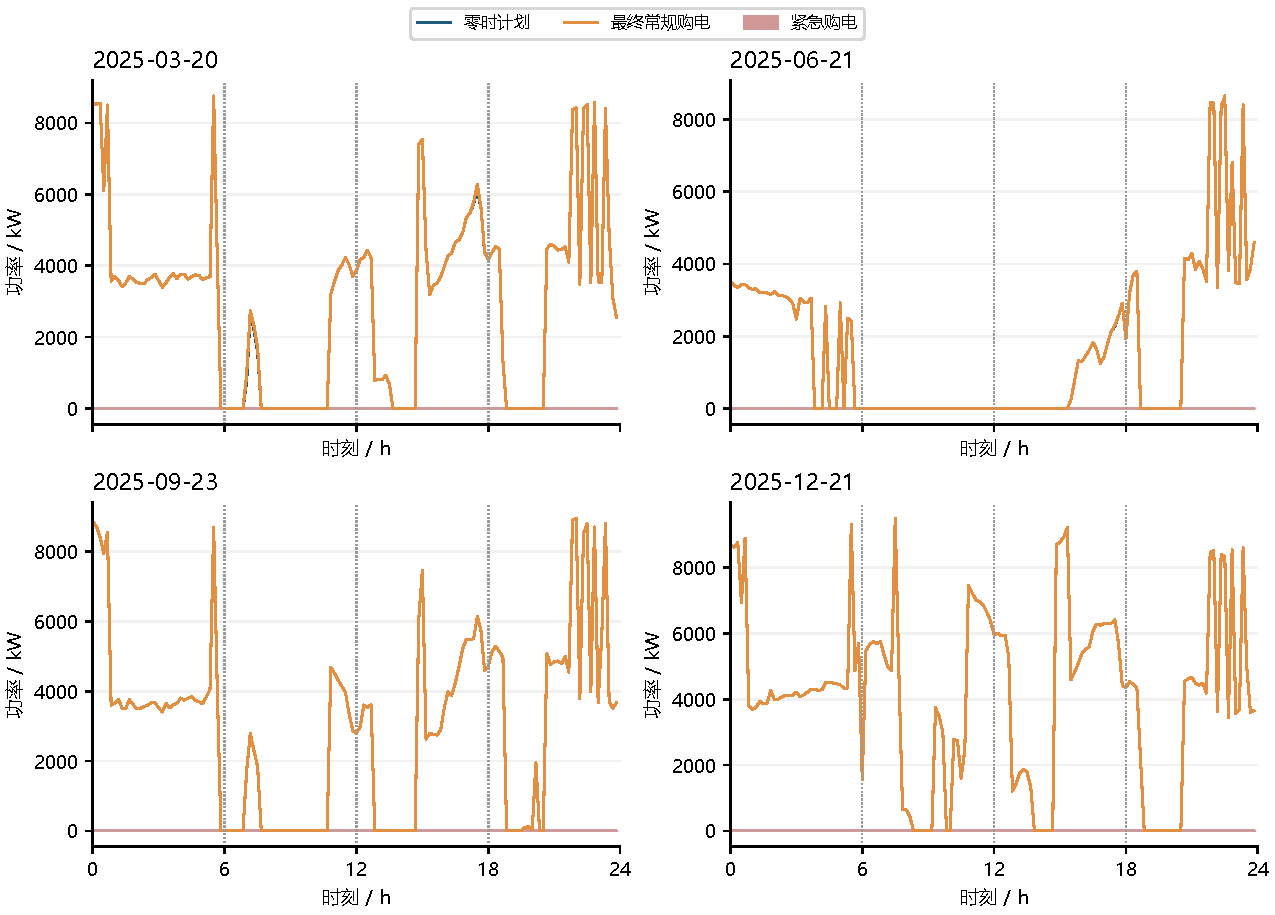
\includegraphics[width=0.96\linewidth]{figures/results/q3_seasons.pdf}
\caption{问题三四个指定日期的计划与执行；虚线表示6、12、18时更新节点}
\label{fig:seasons}
\end{figure}
\FloatBarrier

\subsection{问题四的波动电价结果}

在实际波动电价下，问题四对应问题二的策略总费用为14874522.48元，其中紧急费用477058.06元，紧急电量75130.77 kWh；对应问题三的滚动策略总费用为14871979.24元，其中调整费226405.77元、紧急费60145.05元，紧急电量9795.55 kWh。两者常规计划费用分别为14397464.42元和14585428.42元。

滚动策略节约2543.24元，仅占静态费用的0.017\%，但紧急电量降低86.96\%。这种结果符合题目收费结构：提早锁定较多电量和增加调整交易，能够减少五倍紧急购电，然而常规采购与调整成本抵消了大部分节省。日费用经验CVaR95由81744.59元降至77615.52元，最高日费用由100034.45元降至81371.51元，说明在本年度数据中更明显的收益体现在高费用日期与应急依赖，而非平均总费用的大幅降低。

\begin{table}[htbp]\centering\small
\caption{问题4-2指定日期购电结果（沿用题目表1布局，电量单位：kWh）}
\label{tab:q4_2-purchase}
\par\smallskip\textbf{2025-03-20}\par\smallskip
\begin{tabularx}{\linewidth}{lRlRlR}
\toprule
时间段 & 购电量 & 时间段 & 购电量 & 时间段 & 购电量\\
\midrule
10:00--10:10 & 0.00 & 12:00--12:10 & 634.67 & 14:00--14:10 & 0.00\\
16:00--16:10 & 501.72 & 18:00--18:10 & 0.00 & 20:00--20:10 & 735.49\\
\midrule
全天购电量 & 69863.61 & \multicolumn{2}{c}{全天购电费（元）} & \multicolumn{2}{r}{43714.39}\\
\bottomrule
\end{tabularx}
\par\smallskip\textbf{2025-06-21}\par\smallskip
\begin{tabularx}{\linewidth}{lRlRlR}
\toprule
时间段 & 购电量 & 时间段 & 购电量 & 时间段 & 购电量\\
\midrule
10:00--10:10 & 0.00 & 12:00--12:10 & 0.00 & 14:00--14:10 & 0.00\\
16:00--16:10 & 232.58 & 18:00--18:10 & 533.11 & 20:00--20:10 & 0.00\\
\midrule
全天购电量 & 42111.36 & \multicolumn{2}{c}{全天购电费（元）} & \multicolumn{2}{r}{21455.96}\\
\bottomrule
\end{tabularx}
\par\smallskip\textbf{2025-09-23}\par\smallskip
\begin{tabularx}{\linewidth}{lRlRlR}
\toprule
时间段 & 购电量 & 时间段 & 购电量 & 时间段 & 购电量\\
\midrule
10:00--10:10 & 0.00 & 12:00--12:10 & 588.49 & 14:00--14:10 & 0.00\\
16:00--16:10 & 572.26 & 18:00--18:10 & 0.00 & 20:00--20:10 & 17.80\\
\midrule
全天购电量 & 68805.32 & \multicolumn{2}{c}{全天购电费（元）} & \multicolumn{2}{r}{47789.54}\\
\bottomrule
\end{tabularx}
\par\smallskip\textbf{2025-12-21}\par\smallskip
\begin{tabularx}{\linewidth}{lRlRlR}
\toprule
时间段 & 购电量 & 时间段 & 购电量 & 时间段 & 购电量\\
\midrule
10:00--10:10 & 0.00 & 12:00--12:10 & 987.41 & 14:00--14:10 & 0.00\\
16:00--16:10 & 879.43 & 18:00--18:10 & 731.06 & 20:00--20:10 & 0.00\\
\midrule
全天购电量 & 99329.95 & \multicolumn{2}{c}{全天购电费（元）} & \multicolumn{2}{r}{75678.23}\\
\bottomrule
\end{tabularx}
\par\smallskip\parbox{\linewidth}{\footnotesize 注：问题2与4-2列示计划购电量；问题3与4-3列示最终生效的调整后常规购电量。全天购电量不含紧急购电，全天购电费含计划、调整与紧急费用。}
\end{table}

\begin{table}[htbp]\centering\small
\caption{问题4-2指定日期储能结果（沿用题目表2布局，单位：kWh）}
\label{tab:q4_2-battery}
\par\smallskip\textbf{2025-03-20}\par\smallskip
\begin{tabularx}{\linewidth}{lRRlRR}
\toprule
时间段 & 充电量 & 放电量 & 时间段 & 充电量 & 放电量\\
\midrule
00:00--04:00 & 2173.72 & 175.05 & 04:00--08:00 & 3492.41 & 5061.23\\
08:00--12:00 & 6291.46 & 2777.38 & 12:00--16:00 & 2694.62 & 356.34\\
16:00--20:00 & 191.41 & 6344.65 & 20:00--24:00 & 5580.52 & 2211.32\\
\midrule
0:00储电量 & \multicolumn{2}{r}{6800.10} & 24:00储电量 & \multicolumn{2}{r}{6375.20}\\
\bottomrule
\end{tabularx}
\par\smallskip\textbf{2025-06-21}\par\smallskip
\begin{tabularx}{\linewidth}{lRRlRR}
\toprule
时间段 & 充电量 & 放电量 & 时间段 & 充电量 & 放电量\\
\midrule
00:00--04:00 & 779.63 & 3116.33 & 04:00--08:00 & 2976.61 & 1719.95\\
08:00--12:00 & 5636.01 & 0.00 & 12:00--16:00 & 0.00 & 0.00\\
16:00--20:00 & 0.00 & 4809.67 & 20:00--24:00 & 5846.76 & 2485.90\\
\midrule
0:00储电量 & \multicolumn{2}{r}{7720.62} & 24:00储电量 & \multicolumn{2}{r}{7955.90}\\
\bottomrule
\end{tabularx}
\par\smallskip\textbf{2025-09-23}\par\smallskip
\begin{tabularx}{\linewidth}{lRRlRR}
\toprule
时间段 & 充电量 & 放电量 & 时间段 & 充电量 & 放电量\\
\midrule
00:00--04:00 & 4767.05 & 44.00 & 04:00--08:00 & 99.10 & 5848.24\\
08:00--12:00 & 5319.17 & 1896.62 & 12:00--16:00 & 4406.89 & 479.52\\
16:00--20:00 & 284.97 & 7326.64 & 20:00--24:00 & 5574.69 & 1301.33\\
\midrule
0:00储电量 & \multicolumn{2}{r}{6523.80} & 24:00储电量 & \multicolumn{2}{r}{6156.77}\\
\bottomrule
\end{tabularx}
\par\smallskip\textbf{2025-12-21}\par\smallskip
\begin{tabularx}{\linewidth}{lRRlRR}
\toprule
时间段 & 充电量 & 放电量 & 时间段 & 充电量 & 放电量\\
\midrule
00:00--04:00 & 4574.65 & 75.61 & 04:00--08:00 & 800.60 & 1392.25\\
08:00--12:00 & 5983.94 & 6334.74 & 12:00--16:00 & 5528.51 & 2220.11\\
16:00--20:00 & 7.12 & 5550.99 & 20:00--24:00 & 5691.21 & 2842.53\\
\midrule
0:00储电量 & \multicolumn{2}{r}{6737.42} & 24:00储电量 & \multicolumn{2}{r}{6602.37}\\
\bottomrule
\end{tabularx}
\end{table}

\begin{table}[htbp]\centering\small
\caption{问题4-2指定日期紧急购电（题目表3布局，单位：kWh）}
\label{tab:q4_2-emergency}
\setlength{\tabcolsep}{3pt}
\begin{tabularx}{\linewidth}{lRlRlRlR}\toprule
\multicolumn{2}{c}{2025-03-20} & \multicolumn{2}{c}{2025-06-21} & \multicolumn{2}{c}{2025-09-23} & \multicolumn{2}{c}{2025-12-21}\\
时间段 & 购电量 & 时间段 & 购电量 & 时间段 & 购电量 & 时间段 & 购电量\\\midrule
无 & 0.00 & 无 & 0.00 & 18:20--18:40 & 3.91 & 无 & 0.00\\
 &   &  &   & 20:30--21:00 & 481.54 &  &  \\
\midrule
合计 & 0.00 & 合计 & 0.00 & 合计 & 485.45 & 合计 & 0.00\\
\bottomrule\end{tabularx}\end{table}
\FloatBarrier
\begin{table}[htbp]\centering\small
\caption{问题4-3指定日期购电结果（沿用题目表1布局，电量单位：kWh）}
\label{tab:q4_3-purchase}
\par\smallskip\textbf{2025-03-20}\par\smallskip
\begin{tabularx}{\linewidth}{lRlRlR}
\toprule
时间段 & 购电量 & 时间段 & 购电量 & 时间段 & 购电量\\
\midrule
10:00--10:10 & 0.00 & 12:00--12:10 & 662.11 & 14:00--14:10 & 188.29\\
16:00--16:10 & 680.86 & 18:00--18:10 & 692.66 & 20:00--20:10 & 295.12\\
\midrule
全天购电量 & 71818.10 & \multicolumn{2}{c}{全天购电费（元）} & \multicolumn{2}{r}{45444.10}\\
\bottomrule
\end{tabularx}
\par\smallskip\textbf{2025-06-21}\par\smallskip
\begin{tabularx}{\linewidth}{lRlRlR}
\toprule
时间段 & 购电量 & 时间段 & 购电量 & 时间段 & 购电量\\
\midrule
10:00--10:10 & 0.00 & 12:00--12:10 & 0.00 & 14:00--14:10 & 0.00\\
16:00--16:10 & 216.84 & 18:00--18:10 & 514.10 & 20:00--20:10 & 0.00\\
\midrule
全天购电量 & 37850.75 & \multicolumn{2}{c}{全天购电费（元）} & \multicolumn{2}{r}{19741.04}\\
\bottomrule
\end{tabularx}
\par\smallskip\textbf{2025-09-23}\par\smallskip
\begin{tabularx}{\linewidth}{lRlRlR}
\toprule
时间段 & 购电量 & 时间段 & 购电量 & 时间段 & 购电量\\
\midrule
10:00--10:10 & 13.89 & 12:00--12:10 & 468.91 & 14:00--14:10 & 99.25\\
16:00--16:10 & 590.04 & 18:00--18:10 & 0.00 & 20:00--20:10 & 18.16\\
\midrule
全天购电量 & 73494.01 & \multicolumn{2}{c}{全天购电费（元）} & \multicolumn{2}{r}{48516.22}\\
\bottomrule
\end{tabularx}
\par\smallskip\textbf{2025-12-21}\par\smallskip
\begin{tabularx}{\linewidth}{lRlRlR}
\toprule
时间段 & 购电量 & 时间段 & 购电量 & 时间段 & 购电量\\
\midrule
10:00--10:10 & 0.00 & 12:00--12:10 & 1069.08 & 14:00--14:10 & 0.00\\
16:00--16:10 & 897.85 & 18:00--18:10 & 724.70 & 20:00--20:10 & 0.00\\
\midrule
全天购电量 & 99454.26 & \multicolumn{2}{c}{全天购电费（元）} & \multicolumn{2}{r}{75908.54}\\
\bottomrule
\end{tabularx}
\par\smallskip\parbox{\linewidth}{\footnotesize 注：问题2与4-2列示计划购电量；问题3与4-3列示最终生效的调整后常规购电量。全天购电量不含紧急购电，全天购电费含计划、调整与紧急费用。}
\end{table}

\begin{table}[htbp]\centering\small
\caption{问题4-3指定日期储能结果（沿用题目表2布局，单位：kWh）}
\label{tab:q4_3-battery}
\par\smallskip\textbf{2025-03-20}\par\smallskip
\begin{tabularx}{\linewidth}{lRRlRR}
\toprule
时间段 & 充电量 & 放电量 & 时间段 & 充电量 & 放电量\\
\midrule
00:00--04:00 & 4338.13 & 146.27 & 04:00--08:00 & 464.61 & 6007.86\\
08:00--12:00 & 6075.16 & 2777.38 & 12:00--16:00 & 4821.91 & 236.17\\
16:00--20:00 & 43.48 & 5767.09 & 20:00--24:00 & 5592.11 & 2652.48\\
\midrule
0:00储电量 & \multicolumn{2}{r}{6856.48} & 24:00储电量 & \multicolumn{2}{r}{6516.95}\\
\bottomrule
\end{tabularx}
\par\smallskip\textbf{2025-06-21}\par\smallskip
\begin{tabularx}{\linewidth}{lRRlRR}
\toprule
时间段 & 充电量 & 放电量 & 时间段 & 充电量 & 放电量\\
\midrule
00:00--04:00 & 606.72 & 3861.83 & 04:00--08:00 & 1440.68 & 1719.95\\
08:00--12:00 & 8112.31 & 0.00 & 12:00--16:00 & 0.00 & 0.00\\
16:00--20:00 & 0.00 & 4755.36 & 20:00--24:00 & 6799.43 & 3091.92\\
\midrule
0:00储电量 & \multicolumn{2}{r}{7858.24} & 24:00储电量 & \multicolumn{2}{r}{8200.29}\\
\bottomrule
\end{tabularx}
\par\smallskip\textbf{2025-09-23}\par\smallskip
\begin{tabularx}{\linewidth}{lRRlRR}
\toprule
时间段 & 充电量 & 放电量 & 时间段 & 充电量 & 放电量\\
\midrule
00:00--04:00 & 4735.94 & 72.91 & 04:00--08:00 & 367.84 & 5179.79\\
08:00--12:00 & 6326.29 & 1893.23 & 12:00--16:00 & 2296.37 & 201.04\\
16:00--20:00 & 194.97 & 6015.79 & 20:00--24:00 & 5659.23 & 2603.73\\
\midrule
0:00储电量 & \multicolumn{2}{r}{6609.50} & 24:00储电量 & \multicolumn{2}{r}{6491.54}\\
\bottomrule
\end{tabularx}
\par\smallskip\textbf{2025-12-21}\par\smallskip
\begin{tabularx}{\linewidth}{lRRlRR}
\toprule
时间段 & 充电量 & 放电量 & 时间段 & 充电量 & 放电量\\
\midrule
00:00--04:00 & 4651.42 & 90.02 & 04:00--08:00 & 0.00 & 825.69\\
08:00--12:00 & 6331.05 & 6029.43 & 12:00--16:00 & 4930.50 & 2266.73\\
16:00--20:00 & 0.00 & 5557.59 & 20:00--24:00 & 5703.18 & 2842.53\\
\midrule
0:00储电量 & \multicolumn{2}{r}{6713.74} & 24:00储电量 & \multicolumn{2}{r}{6599.39}\\
\bottomrule
\end{tabularx}
\end{table}

\begin{table}[htbp]\centering\small
\caption{问题4-3指定日期紧急购电（题目表3布局，单位：kWh）}
\label{tab:q4_3-emergency}
\setlength{\tabcolsep}{3pt}
\begin{tabularx}{\linewidth}{lRlRlRlR}\toprule
\multicolumn{2}{c}{2025-03-20} & \multicolumn{2}{c}{2025-06-21} & \multicolumn{2}{c}{2025-09-23} & \multicolumn{2}{c}{2025-12-21}\\
时间段 & 购电量 & 时间段 & 购电量 & 时间段 & 购电量 & 时间段 & 购电量\\\midrule
无 & 0.00 & 无 & 0.00 & 20:10--20:20 & 10.23 & 无 & 0.00\\
\midrule
合计 & 0.00 & 合计 & 0.00 & 合计 & 10.23 & 合计 & 0.00\\
\bottomrule\end{tabularx}\end{table}
\begin{table}[htbp]\centering\small
\caption{问题4-3指定日期计划、调整与费用分解}
\begin{tabularx}{\linewidth}{lRRRRR}\toprule
日期 & 计划量/kWh & 生效量/kWh & 计划费/元 & 调整费/元 & 紧急费/元\\\midrule
2025-03-20 & 71655.38 & 71818.10 & 45192.28 & 251.82 & 0.00\\
2025-06-21 & 37850.75 & 37850.75 & 19741.04 & 0.00 & 0.00\\
2025-09-23 & 73480.32 & 73494.01 & 48421.73 & 28.22 & 66.27\\
2025-12-21 & 99257.81 & 99454.26 & 75595.15 & 313.39 & 0.00\\
\bottomrule\end{tabularx}\end{table}

图\ref{fig:monthly}给出月度费用与紧急量。夏季及冬季的负荷、光伏和价格水平不同，固定电价与波动电价的结果会产生季节性差别。图中全部月份均为样本外顺序结算结果，历史窗口和风险参数不根据这些月份的评价值进行反向选择。

\begin{figure}[htbp]
\centering
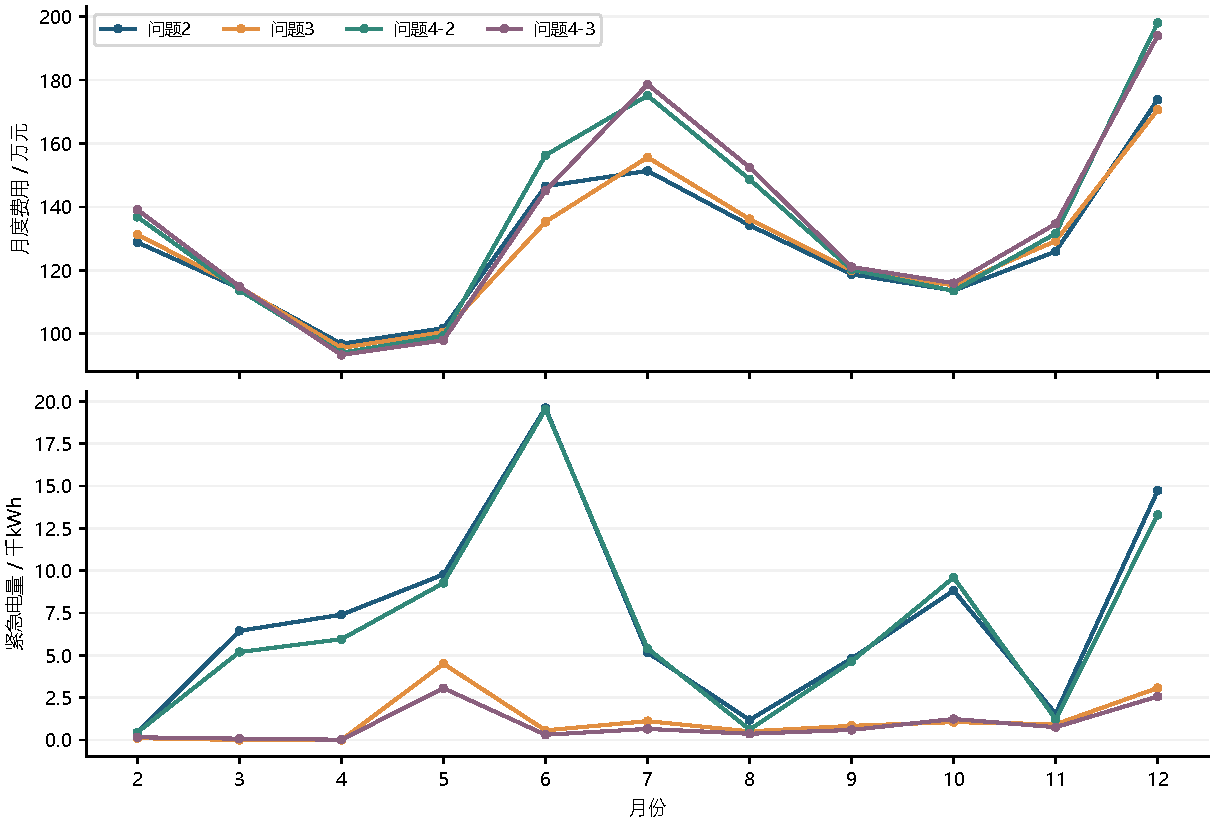
\includegraphics[width=0.94\linewidth]{figures/results/monthly_results.pdf}
\caption{四组策略在评价期内的月度费用与紧急购电量}
\label{fig:monthly}
\end{figure}
\FloatBarrier
